% Title: gl2ps_renderer figure
% Creator: GL2PS 1.4.0, (C) 1999-2017 C. Geuzaine
% For: Octave
% CreationDate: Tue Oct 26 18:08:16 2021
\setlength{\unitlength}{1pt}
\begin{picture}(0,0)
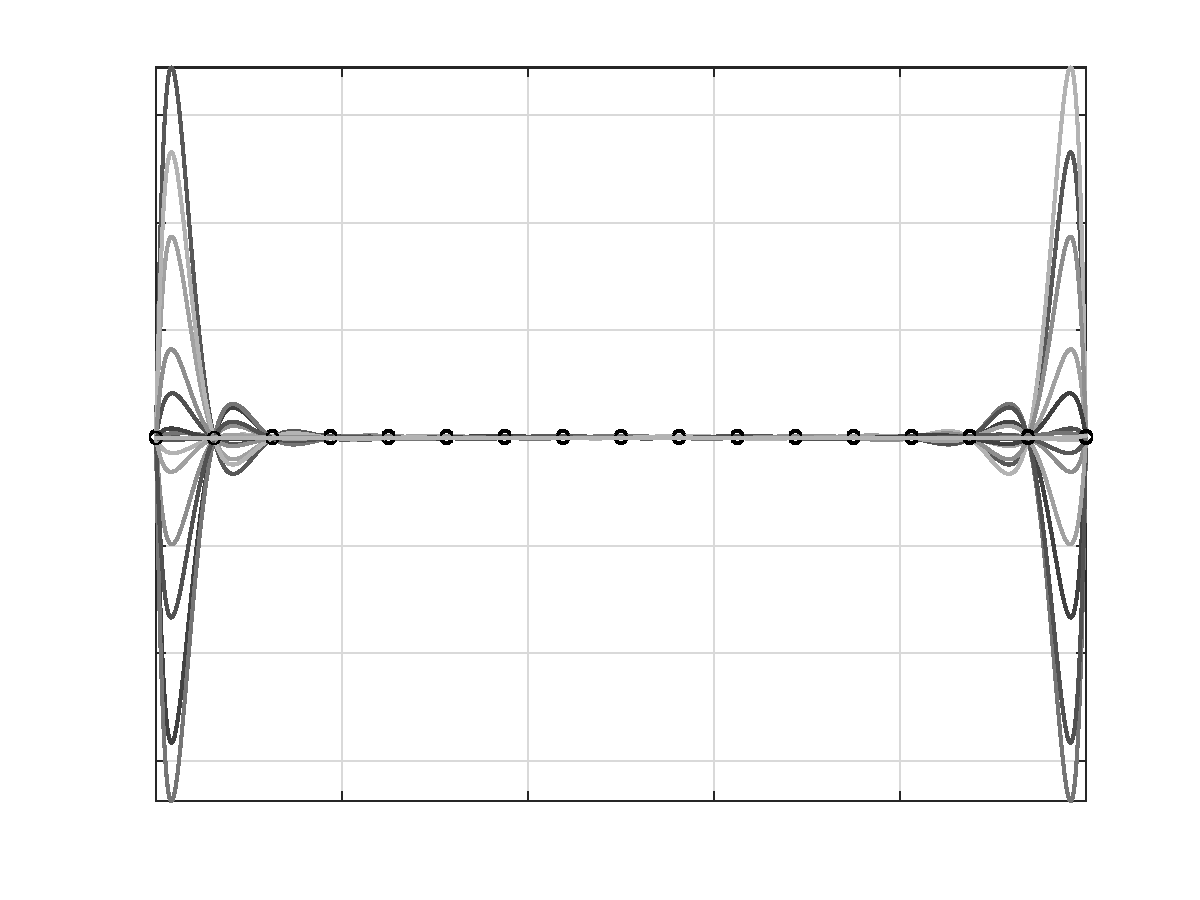
\includegraphics{figures/chap10/OUT/Basis016UniformGray-inc}
\end{picture}%
\begin{picture}(576,432)(0,0)
\fontsize{10}{0}
\selectfont\put(74.88,40.0183){\makebox(0,0)[t]{\textcolor[rgb]{0.15,0.15,0.15}{{0}}}}
\fontsize{10}{0}
\selectfont\put(164.16,40.0183){\makebox(0,0)[t]{\textcolor[rgb]{0.15,0.15,0.15}{{0.2}}}}
\fontsize{10}{0}
\selectfont\put(253.44,40.0183){\makebox(0,0)[t]{\textcolor[rgb]{0.15,0.15,0.15}{{0.4}}}}
\fontsize{10}{0}
\selectfont\put(342.72,40.0183){\makebox(0,0)[t]{\textcolor[rgb]{0.15,0.15,0.15}{{0.6}}}}
\fontsize{10}{0}
\selectfont\put(432,40.0183){\makebox(0,0)[t]{\textcolor[rgb]{0.15,0.15,0.15}{{0.8}}}}
\fontsize{10}{0}
\selectfont\put(521.28,40.0183){\makebox(0,0)[t]{\textcolor[rgb]{0.15,0.15,0.15}{{1}}}}
\fontsize{10}{0}
\selectfont\put(69.8755,66.848){\makebox(0,0)[r]{\textcolor[rgb]{0.15,0.15,0.15}{{-150}}}}
\fontsize{10}{0}
\selectfont\put(69.8755,118.479){\makebox(0,0)[r]{\textcolor[rgb]{0.15,0.15,0.15}{{-100}}}}
\fontsize{10}{0}
\selectfont\put(69.8755,170.111){\makebox(0,0)[r]{\textcolor[rgb]{0.15,0.15,0.15}{{-50}}}}
\fontsize{10}{0}
\selectfont\put(69.8755,221.742){\makebox(0,0)[r]{\textcolor[rgb]{0.15,0.15,0.15}{{0}}}}
\fontsize{10}{0}
\selectfont\put(69.8755,273.373){\makebox(0,0)[r]{\textcolor[rgb]{0.15,0.15,0.15}{{50}}}}
\fontsize{10}{0}
\selectfont\put(69.8755,325.004){\makebox(0,0)[r]{\textcolor[rgb]{0.15,0.15,0.15}{{100}}}}
\fontsize{10}{0}
\selectfont\put(69.8755,376.636){\makebox(0,0)[r]{\textcolor[rgb]{0.15,0.15,0.15}{{150}}}}
\fontsize{11}{0}
\selectfont\put(298.08,409.6){\makebox(0,0)[b]{\textcolor[rgb]{0,0,0}{{Lagrange Basis Functions of Degree 16: Uniform Nodes}}}}
\fontsize{11}{0}
\selectfont\put(298.08,27.0183){\makebox(0,0)[t]{\textcolor[rgb]{0.15,0.15,0.15}{{x}}}}
\end{picture}
